
텍스트 $T[1..n]$ 

패턴 $P[1..m]$

$\Sigma$ : 문자열에 사용되는 알파벳 집합 

\section{The naive string-matching algorithm}

\begin{itemize}
    \item 전처리 0 
    \item 매칭시간 $O((n-m+1)m)$
    
\end{itemize}

가장간단하면서 일반적으로 생각할수있는 방법이다.
각 $k$마다 $T[k]$부터 $T[k+m-1]$까지 하나하나 $P$와 맞는지 확인하는것이다.

\begin{lstlisting}[style = CStyle]
NAIVE-STRING-MATCHER (T,P)
    n = T.length
    m = P.length
    for s = 0 to n-m
        if(P[1..m] == T[s+1..s+m])
            print ``Pattern occurs with shift s"
\end{lstlisting}



\section{The Rabin-Karp algorithm}
\begin{itemize}
    \item 전처리 $\Theta(m)$
    \item 매칭시간 $O((n-m+1)m)$
\end{itemize}

\begin{figure}[h!]
    \centering
    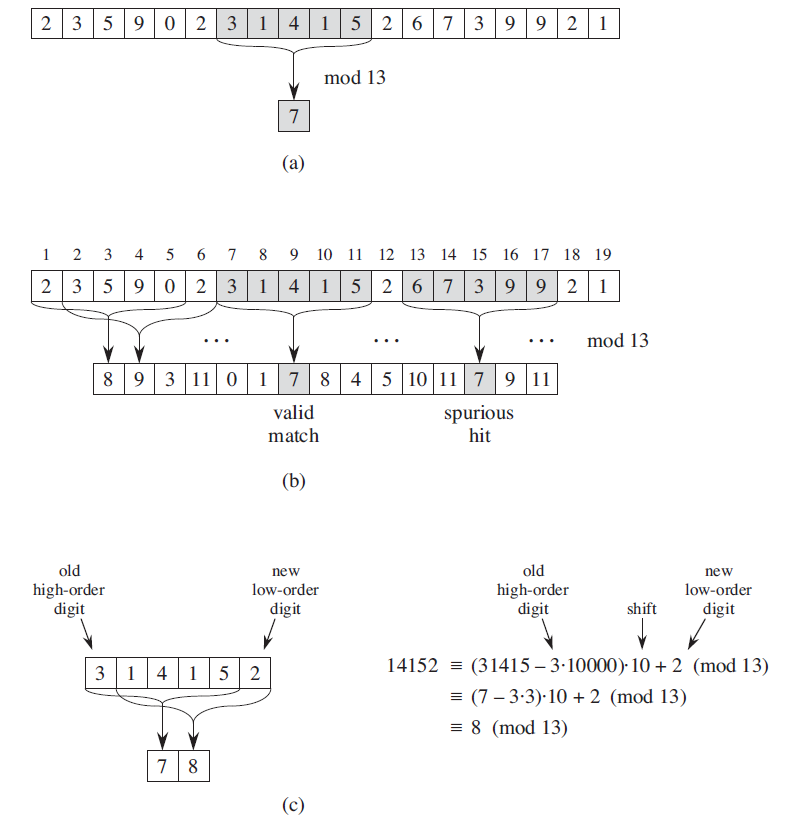
\includegraphics[scale=0.6]{./string_matching/pic1.PNG}
    \caption{$d = 10$, $q = 13$에 대한 라빈카프 알고리즘에 대한 수행을 나타낸다. (a)는 ``31415"에 대한 t가 7인모습 (b)는 숫자가 겹치지만 서로 다른 문자열에 대한것 (c)는 숫자비교를 끝낸후 다음 문자열에대한 변환을 나타낸 것이다.}
\end{figure}


수행시간을 개선하는 첫번째 아이디어는 문자를 숫자로 바꾸는것이다.
$111$과 $121$이란 문자열을 비교하려면 첫번째방법인 각 자리별로 3번 비교해야하지만 숫자로 비교하는건 한번만 비교하면된다.
따라서 문자열을 숫자로 바꾸기위한 전처리 시간이 든다.
전처리는 $P$패턴만을 $\Theta(m)$동안 바꾸고 문자열 $T$는 비교와 동시에 처리한다.

그다음 문자열을 어떻게 숫자로 나타낼까를 고민해야하는데 이때 문자가 나타내는 언어의 총갯수에대한 진법에서 10진법으로 변환한다. 따라서 실제 알고리즘을 실행할때 언어의 총갯수 $d$ $(|\Sigma|)$를 인자로 넣어주어야한다.
이때 숫자로 바꿀때 너무 긴 문자열을 숫자로 바꿀시에 나타나는 오버플로우를 감안해, 적당한 값으로 나눌 $q$를 채용한다.그래서 그 나타낸 숫자가 매칭이 이루어졌을때 실제로 같은 문자열인지 검사하는 부분이 필요하다. 이 $q$는 일반적으로 $dq$가 컴퓨터 한워드에 들어가는 소수로 채용한다.

호너의 법칙(Horner's law)을 사용해 다음의 수식으로 $\Theta(m)$시간에 패턴 $P$에대한 숫자 $p$를 전처리한다.

$$p = (dp+P[i]) \bmod q$$

문자열 $T[s+1..s+m]$에 대한 숫자 $t_s$의 처리는 매칭과 직후에 계산 한다.

$$t_{s+1} = (d(t_s - T[s+1]h) + T[s+m+1]) \bmod q$$

$ h = d^{m-1} \bmod q$이다. 가장 앞의 $T[s+1]$을 $h$를 곱해 제거하고 왼쪽으로 시프트 후 $T[s+m+1]$를 더하는 방식이다.



\begin{lstlisting}[style = CStyle]
RABIN-KARP-MATCHER(T,P,d,q)
    n = T.length
    m = P.length
    h = d^{m-1} mod q
    p = 0
    t_0 = 0
    for( i = 1 to m)
        p = (dp+P[i])mod q
        t_0 = (dt_0 + T[i]) mod q
    for s = 0 to n-m
        if p == t_s
            if P[1..m] == T[s+1..s+m]
                print ``Pattern occurs with shift s"
        if s < n - m
            t_{s+1} = (d(t_s - T[s+1]h) + T[s+m+1]) mod q
\end{lstlisting}

이 방법은 초기보다는 확실하게 개선되었지만 여전히 완벽하게 일치하는지 확인하기 위해 하나하나 비교하는 방법을 사용한다. 이상적인 경우는 $(m-n+a)$정도 돌겠지만  따라서 최악의 경우 매칭 시간이 $O((n-m+1)m)$이 된다.

\section{String matching with finite automata}

\begin{itemize}
    \item 전처리 $O(m|\Sigma|)$
    \item 매칭시간 $\Theta(n)$
\end{itemize}

\begin{dfn}[automata]
    finite automaton은 다음과 같이 5개의 튜플로 구성된다.
    \begin{itemize}
        \item $Q$ : 유한 상태의 집합
        \item $q_0$ :시작 상태 ($q_0 \in Q$)
        \item $A$ : 받아들이는 상태의 구분된 상태 ($A \subset Q$)
        \item $\Sigma$ : 유한 입력 알파벳
        \item $\delta$ : $Q \times \Sigma$에서 $Q$로 매핑되는 전이 함수 $M$    \end{itemize}
\end{dfn}

CLRS의 번역본을 그대로 들고왔습니다.


뭔소린지모르겠죠?

저도 그럼

오토마타 내용 통째로 생략

\newpage



\begin{figure}[h!]
    \centering
    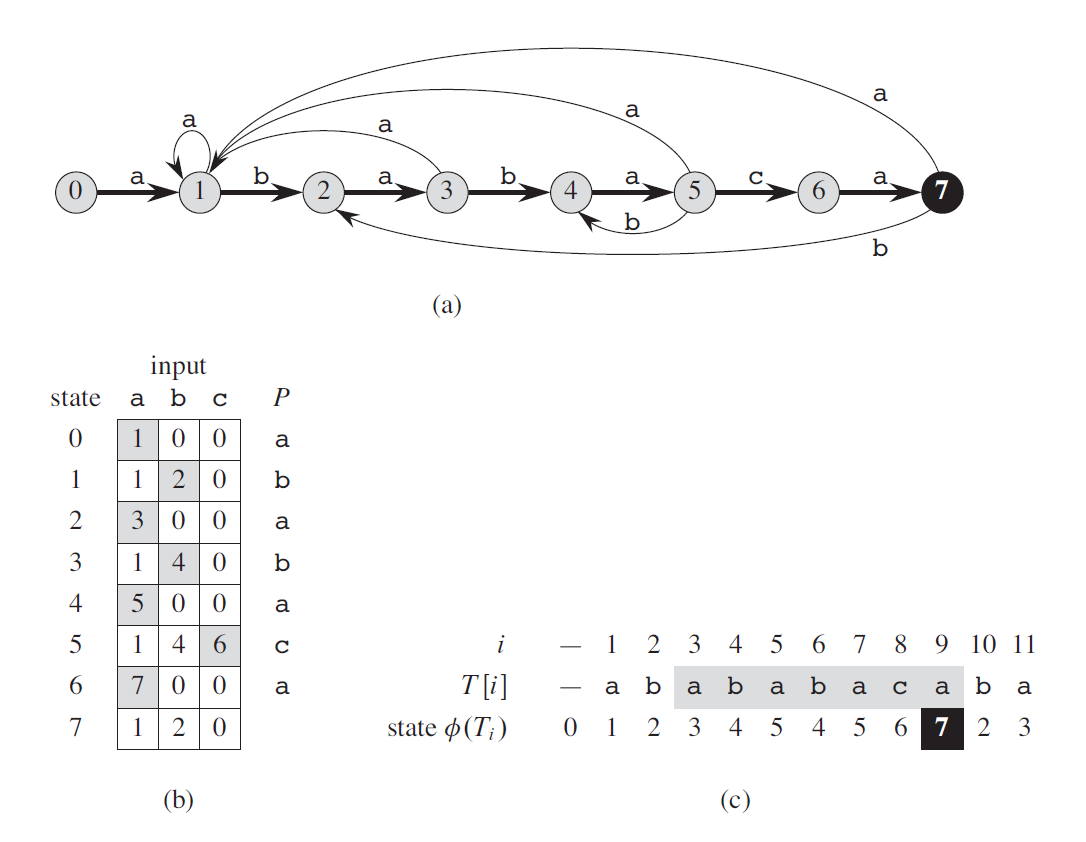
\includegraphics[scale=0.4]{./string_matching/pic2.PNG}
    \caption{$|\Sigma|  = 3$ ``a,b,c", $m = 7$에 대한 스트링 매칭 오토마타
    (a) 패턴 $P$에 대한 상태 오토마타 (b) 상태표 (c) 상태표에 따른 연산}
\end{figure}

오토마타를 이용한 스트링 매칭은 전처리에 일치한 앞 문자열 상태에 따른 상태표 $\delta$를 구하고 이를 이용해 매칭을 하는것이다.
상태는 $0,..,m$까지 있다. 초기 시작 상태는 0이고(매칭되는 알파벳이 하나도 없는 상태)
매칭되는 알파벳갯수에따라 상태 넘버를 가진다.

매칭시에 문자열 $T$는 각 자리마다 상태를 가진다. 각 상태를 가지고 다음에 나오는 문자에 따라 상태를 변화시키고 상태가 $m$에 도달하면 매칭이 된것으로 본다.

상태표의 특징은 상태가 변할때 일치한 문자열이 가장 길게 일치하는 상태로 보내는 것이다.
가령 그림 (c)에서 $T[5]$에서 $T[6]$으로 넘어갈때 ``ababa"까지 일치했지만 ``b"가 나옴으로써 매칭이 실패하지만 뒤에나온 ``b"를 포함해 ``abab"까지가 일치하기에 상태가 4로 돌아간것을 볼수있다.

\begin{lstlisting}[style = CStyle]
FINITE-AUTOMATON-MATCHER(T, delta , m)
n = T.length
q = 0 
for i = 1 to n
    q = d(q,T[i])
    if q == m
        print ``Pattern occurs with shift i-m"
\end{lstlisting}


상태표를 구하기위해서 다음과 같이 진행한다.
각 상태 $q$ 마다 각 알파벳 $a$를 뽑는다.
현재 상태 $q$의 문자열 + 'a'가 임의의 상태 $k$를 끝에서 포함하는지 검사하고 다를시 $k$를 계속 낮춰간다.

\begin{lstlisting}[style = CStyle]
COMPUTE-TRANSITION-FUNCTION(P, Sigma)
m = P.length
for q = 0 to m
    for a in Sigma
        k = min(m+1,q+2)
        repeat 
            k = k - 1
            until P_k ] P_q-a
            d(q,a) = k
return d
\end{lstlisting}



다음의 전처리의 수행시간은  $O(m^3 \Sigma)$이다.
뒷절의 $KMP$방식을 차용해서 $O(m \Sigma)$로 개선할수있다.


라빈 카프보다 확실히 개선된 방안을 가졌으며 전처리에 문자열 $T$의 개입또한 없다. 그러나 위의 전처리 시간은 $O(m^3 \Sigma)$이며, 상태표의 공간 복잡도의 크기가 $\Theta(m|\Sigma|)$만큼 필요하다.
다음 절에서 이를 더 줄여볼것이다.






\section{The Knuth-Morris-Pratt algorithm}

\begin{itemize}
    \item 전처리 : $O(m)$
    \item 매칭시간 : $\Theta(n)$
\end{itemize}


흔히 KMP 알고리즘이라 부르는데 이 알고리즘은 처음의 가장 기본적인 비교방식을 개선했다고 볼 수 있다. 전처리를 통해 계산한 $\pi[1..m]$ 배열을 사용하며, 매칭이 실패했을때, $\pi$배열을 사용한다.
\newpage
\begin{figure}[h!]
    \centering
    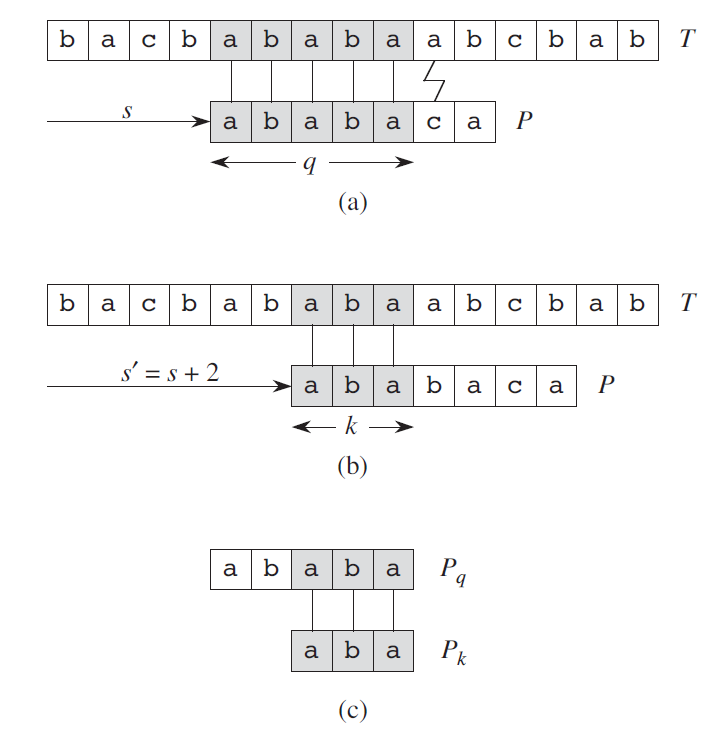
\includegraphics[scale=0.7]{./string_matching/pic3.PNG}
    %\caption{}
\end{figure}

그림과 같이 ``ababaca"패턴을 문자열과 비교한다고 생각해보자.
``ababa"까지 맞지만 'c'와 문자가 일치하지 않는다. 이때 앞의 문자열은 ``ababa"가 패턴이 일치하는것은 자명하다. 이때 ``ababa"에 가장 근접하고 일치하는 수가 적은 $P$의 패턴이 ``aba"임을 알수있는 배열 $\pi[]$를 이용해서 다시 비교하지 않아도 ``aba"까지 일치함을 알수있다. 


\begin{figure}[h!]
    \centering
    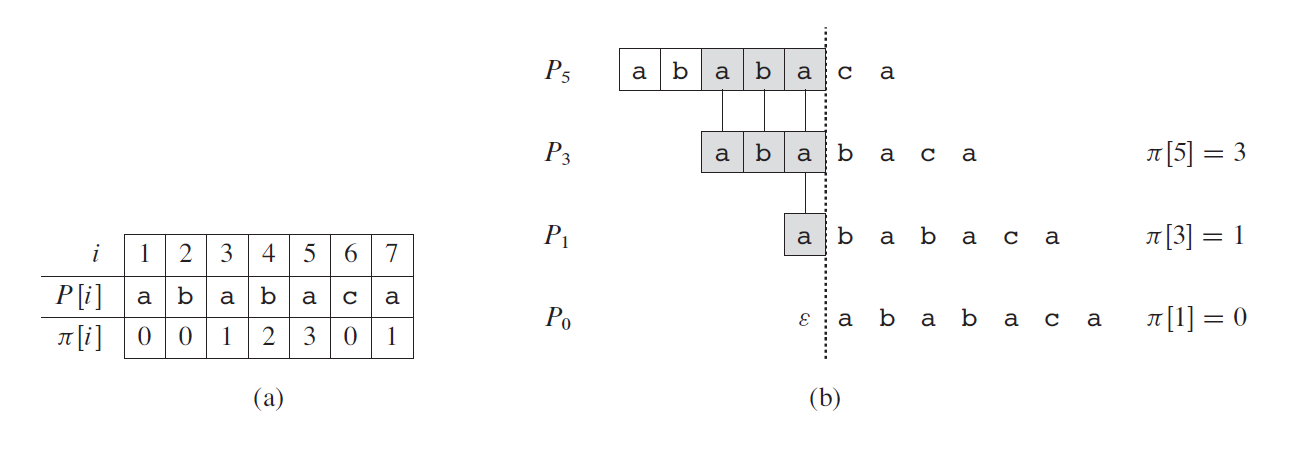
\includegraphics[scale=0.4]{./string_matching/pic4.PNG}
    \caption{(a)는 패턴 $P$와 전처리한 $\pi[1..7]$ (b)는 $P[5]$에서 다음 문자가 매칭이 틀렸을때 그에 따른 $\pi$값과 되돌아가는 순서를 나타낸것이다.}
\end{figure}


\begin{lstlisting}[style = CStyle]
KMP-MATCHER(T,P)
    n = T.length
    m = P:length
    PI[] = COMPUTE-PREFIX-FUNCTION(P)
    q = 0 // number of characters matched
    for i = 1 to n // scan the text from left to right
        while q>0 and P [q+1] != T[i]
            q = PI[q] // next character does not match  
        if P [q+1] == T[i]
            q = q + 1 // next character matches
        if q == m // is all of P matched?
            print ``Pattern occurs with shift" i - m
            q  = PI[q]
\end{lstlisting}



\begin{lstlisting}[style = CStyle]
COMPUTE-PREFIX-FUNCTION(P) /
m = P.length
let PI[1..m] be a new array
PI[1] = 0
k = 0
for q = 2 to m
    while k>0 and P[k+1] != P[q]
        k = P[k]
    if P[k+1] == P[q]
            k = k + 1
    PI[q] = k 
retunr PI
\end{lstlisting}
